\chapter{Chances to Discover Circumbinary Object}
\label{Chapter3}

Chances to discover a circumbinary substellar body depend primarily on three factors: 
\begin{itemize}[noitemsep]
\item the precision and number of the minima which can be achieved;
\item the semi-amplitude of the LITE caused by the body;
\item the intrinsic variability of the binary causing noise in minima timings.
\end{itemize}
%(i) the precision and number of the minima which can be achieved;
%(ii) the semi-amplitude of the LITE caused by the body;
%(iii) the intrinsic variability of the binary causing noise in minima timings.

\section{Precision of the Minimum Time}
The precision of the minimum time $\Delta$t (for a triangular shape of the minimum) can be determined from equation (see, e.g., \cite{sybilski2010})

\begin{equation}\label{eq:dt}
\Delta t = \dfrac{D \sigma}{2d\sqrt{N}}
\end{equation}
where $\sigma$ is the brightness uncertainty (in magnitudes) of a single observational point, $D$ is the duration of the minimum, $d$ is the depth (in magnitudes) and $N$ is the number of observational points during the eclipse. 
The above relation shows that the precision of the minimum time increases with the number of data points taken in the minimum and their precision. The shape of the minimum also affects the precision of the timing -- deep and narrow minima provide the best precision.

In Table \ref{tb:lite_dt} calculated precision for 60 cm telescope of selected as example EB is presented, where $V$ is the out-of-eclipse brightness of the binary, $M_{1,2}$ -- masses of the component, $D$ -- duration of the primary eclipse, $d_{I}, d_{II}$ are the depths of primary and secondary minima, respectively, $\Delta T$ is the amplitude of the LITE for 1 Jupiter mass planet orbiting the binary on a 10 years orbit,
$\Delta t$ -- theoretically achievable primary minimum precision for a 60 cm telescope. 
On Fig.\ref{fig:4_depend} vertical black dash line is corresponding to the mean value of $\Delta t$ calculated for target list from \cite{Pribula2012},~ $\overline{\Delta t} = 2.8$ ~seconds.

\section{Amplitude of LITE Effect}
In case when an unseen third component revolves an EB, the residuals with respect to a linear (or quadratic) ephemeris will show
a wavelike behaviour in the O-C diagram because of the LITE.

The O-C curve (due only to the inner binary) can be described by a linear (constant period) or quadratic
ephemeris (linear period variation) and if a third body is orbiting the inner binary adding the LITE effect, the times
of the minima can be computed from equation (\ref{eq:P_lin_OC_sin}) from Chapter \ref{Chapter_oc}. 
%(a quadratic ephemeris added to the theoretical LITE given by formula (2) and (3) of \cite{irwin1959}).

%\begin{equation}\label{eq:4_minima}
%T_{min} = JD_{0}+P \times E + Q \times E^2 + \dfrac{a_{12}\sin i}{c}   \left[  \dfrac{1-e^2}{1+e \cos\nu}   \sin(\nu + \omega)  + e \sin \omega  \right] 
%\end{equation}

%where $a_{12} \sin i$ is the projected semi-major axis (inclination cannot be derived from the LITE alone), $e$ is the eccentricity,
%$\omega$ is the longitude of the periastron, $\nu$ is the true anomaly of the EB orbit around the common center of the mass of
%the whole system, $JD_{0} + P \times E + Q \times E^2$ is the quadratic ephemeris of the minima of the EB and $c$ is the velocity
%of light. The parameter $Q$ is the coefficient of the quadratic term and gives the rate of the orbital period change of the EB.

\begin{table}[!t]
 \centering
% \small
 \caption{Expected LITE amplitude for Jupiter-mass companion on 15-years orbit and theoretical precision for 60 cm telescope \citep{Pribula2012}.}
 \label{tb:lite_dt}
 \vspace*{1ex}
 \scalebox{1.0}{
 \begin{tabular}{c||c|c|c|c|c|c|c|c}\small
%   Star        &  V   & $M_{1}[M_{\odot}]$ & $M_{2}[M_{\odot}]$ &  $d_{1}[mag]$ & $d_{2}[mag]$ & $D[days]$ & $\Delta ~T[s]$ & $\Delta ~t[s]$ \\
   Star             &  V   & $M_{1}$       & $M_{2}$       &  $d_{I}$ & $d_{II}$ & $D$    & $\Delta T$ & $\Delta t$ \\
                    &  mag & $[M_{\odot}]$ & $[M_{\odot}]$ &  [mag]   & [mag]    & [days] & [s]         & [s] \\
\hline
DV Psc              & 10.6  & 0.49 & 0.51  &  0.32 & 0.15 & 0.062  & 4.5            & 1.1    \\
BX Tri              & 13.4  & 0.51 & 0.26  &  0.33 & 0.27 & 0.072  & 5.4            & 4.2     \\
V470 Cam            & 14.7  & 0.48 & 0.13  &  1.00 & 0.20 & 0.015  & 6.3            & 1.2     \\
GSC 19411746        & 12.9  & 0.56 & 0.65  &  0.90 & 0.40 & 0.453  & 5.1            & 6.1      \\
NY Vir              & 13.3  & 0.50 & 0.15  &  0.90 & 0.15 & 0.012  & 6.0            & 0.6   \\
NSVS 02502726       & 14.0  & 0.71 & 0.35  &  0.50 & 0.35 & 0.084  & 4.3            & 3.9    \\
NSVS 06507557       & 13.4  & 0.66 & 0.28  &  0.70 & 0.23 & 0.062  & 4.7            & 1.8    \\
MR Del              & 11.0  & 0.69 & 0.63  &  0.33 & 0.17 & 0.073  & 3.7            & 1.4      \\
\hline
 \end{tabular}}
\end{table}

The full amplitude of the expected LITE changes caused by another body orbiting a binary on the edge-on (i $\sim$ 90\degree ) circular orbit (e $\sim$ 0\degree) is:

\begin{equation}\label{eq:dT}
\Delta T = \dfrac{2M_{3}G^{1/3}}{c} \left[    \dfrac{P_{3}}{ 2 \pi \left( M_{1}+M_{2} \right) }   \right]^{2/3} 
\end{equation}
where $M_{1} , M_{2} , M_{3}$ are the masses of the components, $G$ is the gravitational constant, $c$ is the speed of light, 
and $P_{3}$ is the orbital period of the third (sub-stellar) component. Equation (\ref{eq:dT}) shows that the semi-amplitude of the LITE
changes is proportional to the mass of the third component and nearly proportional to its orbital period \citep{Pribula2012}. 
Amplitude of LITE effect depends on value of inclination $i$, so if it is less then $90\degree$, $\Delta T$ is decreasing too.   
Calculated value of $\Delta T$ for some binary systems is presented in Table \ref{tb:lite_dt}. 

Full amplitude of LITE effect from period of $3^{rd}$ body dependence is presented graphically on Fig.\ref{fig:4_depend}. %, \ref{fig:4_depend2}.

\begin{figure}[!ht]
\vspace{0cm}
\centerline{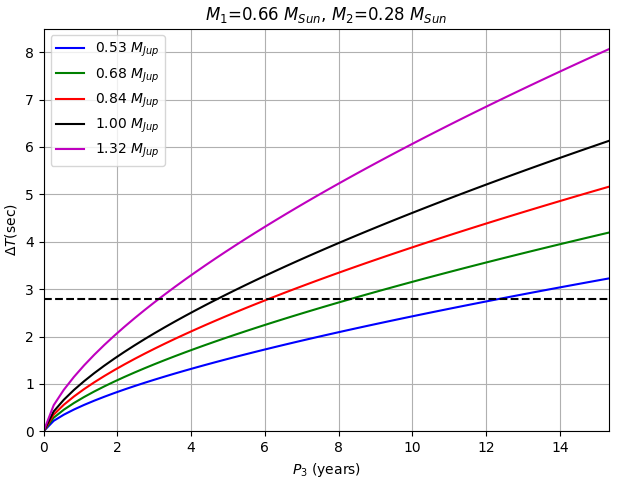
\includegraphics[width=0.8\textwidth,angle=0] {M3_dep_P_1.png}}
\centerline{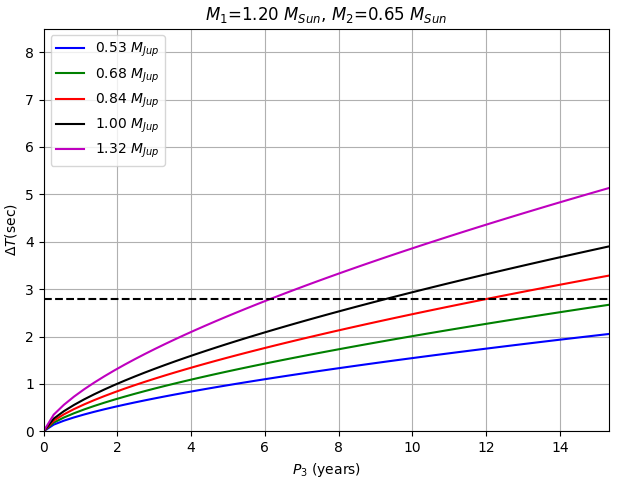
\includegraphics[width=0.8\textwidth,angle=0] {M3_dep_P_3.png}}
\caption{Amplitude of the expected LITE effect $\Delta T$ as the dependence of period of $3^{rd}$ body $P_{3}$. Different masses of third body $M_{3}$ in Jupiter masses is presented by different colours. Vertical dash line is a mean value of theoretical precision of minima $\Delta t$. 
Two graphs for different system components ($M_{1}, M_{2}$).}
\label{fig:4_depend}
\end{figure}

%\begin{figure}[!ht]
%\vspace{0cm}
%\centerline{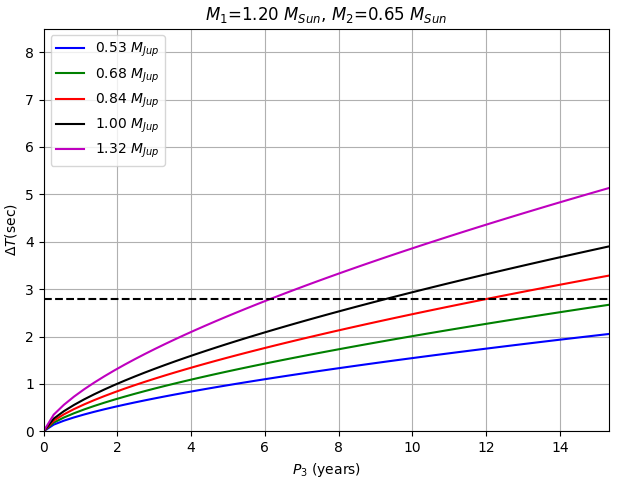
\includegraphics[width=0.8\textwidth,angle=0] {M3_dep_P_3.png}}
%\caption{Amplitude of the expected LITE effect $\Delta T$ as the dependence of period of third body $P_{3}$.  Different masses of third body $M_{3}$ in Jupiter masses is presented by different colours. Vertical dash line is a mean value of theoretical precision of minima $\Delta t$.}
%\label{fig:4_depend2}
%\end{figure}

As can be seen from graphs, minimum amplitude from LITE that can be registered by ~$\sim$ half meter telescope corresponds to one Jupiter mass body or force us to observe binary system on very long time intervals (>15 year). Otherwise, in case of Kepler EB catalogue we have magnitude precision $10^{-6}$, larger diameter, brightness uncertainty $\sigma$ and sometimes more points on minima, that can decrease value of theoretical minima precision $\Delta t$ and allow us to define exoplanets or brown dwarfs in eclipsing binary systems with masses of third body less then one Jupiter mass.  

\section{Building O-C Diagrams from Kepler Data}
Kepler satellite provides us with unprecedented accuracy of photometric data.
Such a huge database of EBs observed with high precision and monitored continuously over a period of several years
encouraged several teams to look for a periodic modulation of data, indicative of multiple systems.  
For example, \cite{gies2012} presented 41 suspected triples, while \cite{conroy2014} listed 236
potential triples. Moreover, \cite{Rappaport2013} presented 39 dynamically interesting systems, where
the third-body periods are short enough (if compared with the binary period) that some interaction between the orbits is
expected or even observed (e.g., changing of the inclination).
On the other hand, most of the triples listed in \cite{conroy2014} have periods of the order of hundreds or even thousands
of days, so long periods were usually only estimated (due to limited coverage of the Kepler data) or were influenced by
large errors \citep{Zasche2015}.

For this reason, we decided to perform a similar analysis to detect circumbinary objects for other systems, but based on a
larger data set if available, and taking into account different phenomena that distort EBs light curve.

In order to define the time of minima from available light curve in Kepler EB catalogue, special python script was written. 
This algorithm reads Kepler input catalog ID (KIC), period and initial epoch of binary system from Kepler EB catalogue. According to obtained KIC, we check if ~short or long cadence data, or both of them, are available, and start to process this light data.

In order to find the exact time of minima different methods can be used, most popular of them are described in Chapter \ref{Chapter_minima_det}. In this preliminary analysis we use fitting with Lorentz function (see equation \ref{eq:lorentz}) because it is simple method with good accuracy. In dissertation thesis we plan to compare mentioned methods and the best one will be used. Using Lorentz function we do not fit whole light curve, only the minimum part, for primary minimum we use only data with phase in range $-0.25 < \varphi < 0.25$.

Also, we can cut upper part of LC, for example taking into account only 70\%~-~90\% of LC amplitude, such approach increase fit precision. This is demonstrated on Fig.\ref{fig:ind_min_fit},\ref{fig:ind_min_fit2}. The only warning, in such approach, is to get enough data points because, as we know, precision of minima also depends on number of used points. 
\begin{figure}[!t]
\vspace{0cm}
\begin{tabular}{ll}
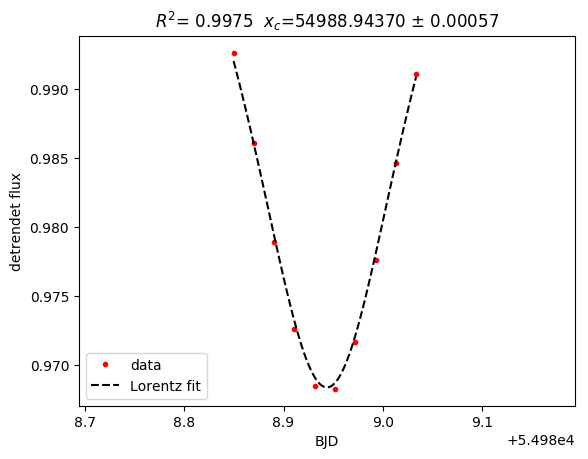
\includegraphics[width=.49\textwidth,angle=0] {lor/54988_9437025_08.png}
&
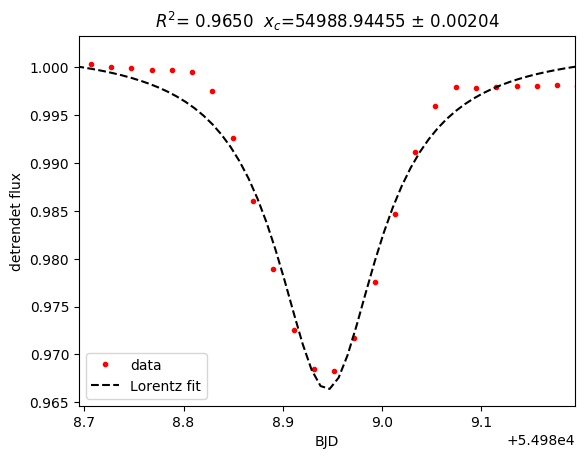
\includegraphics[width=.49\textwidth,angle=0] {lor/54988_9445532_1.png}
\end{tabular}
\caption{Individual minima fit (dashed line) of KIC 4681152 primary minima. Same minima fitted on two figures. Left: 80\% of amplitude Right: 100\% of amplitude}
\label{fig:ind_min_fit}
\end{figure}
\begin{figure}[!t]
\vspace{0cm}
\begin{tabular}{ll}
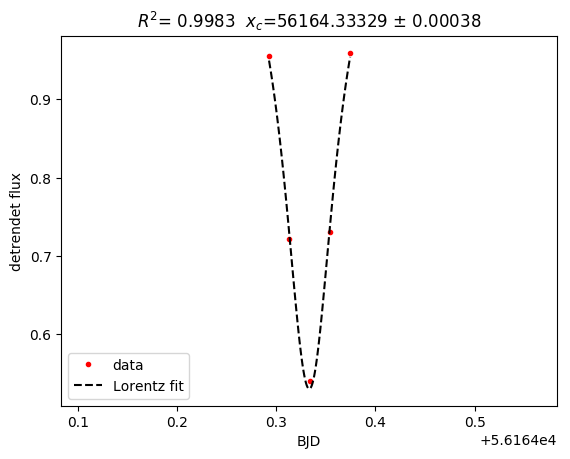
\includegraphics[width=.49\textwidth,angle=0] {lor/2/85_56164_3332913.png}
&
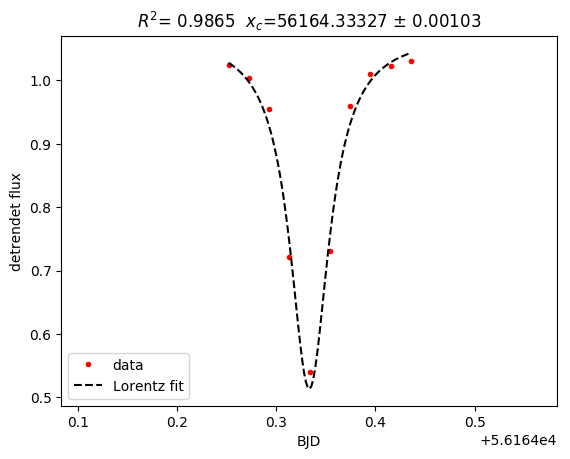
\includegraphics[width=.49\textwidth,angle=0] {lor/2/100_56164_3332725.png}
\end{tabular}
\caption{Individual minima fit (dashed line) of KIC 12553806 primary minima. Same minima fitted on two figures. Left: 85\% of amplitude Right: 100\% of amplitude}
\label{fig:ind_min_fit2}
\end{figure}

On the final stage, new ephemeris is computed and O-C diagram is formed from obtained times of minima. Some of these O-C diagrams are presented on Fig.\ref{fig:oc}. Having precessed, in such way, all binary systems in Kepler EB catalogue we have highlighted, in a first approximation, 169 systems with possible circumbinary objects or other physical phenomenons that are appearing on O-C diagrams. Some of these binary systems are highlighted for sure, and in many cases good detected systems are marked as multiple previously in works of ~\cite{gies2012, Rappaport2013, conroy2014}. There is also lot of candidates which will be studied more accurately with considering of other factors influence.   
\begin{figure}[!th] 
  \begin{subfigure}[b]{0.5\linewidth}
    \centering
    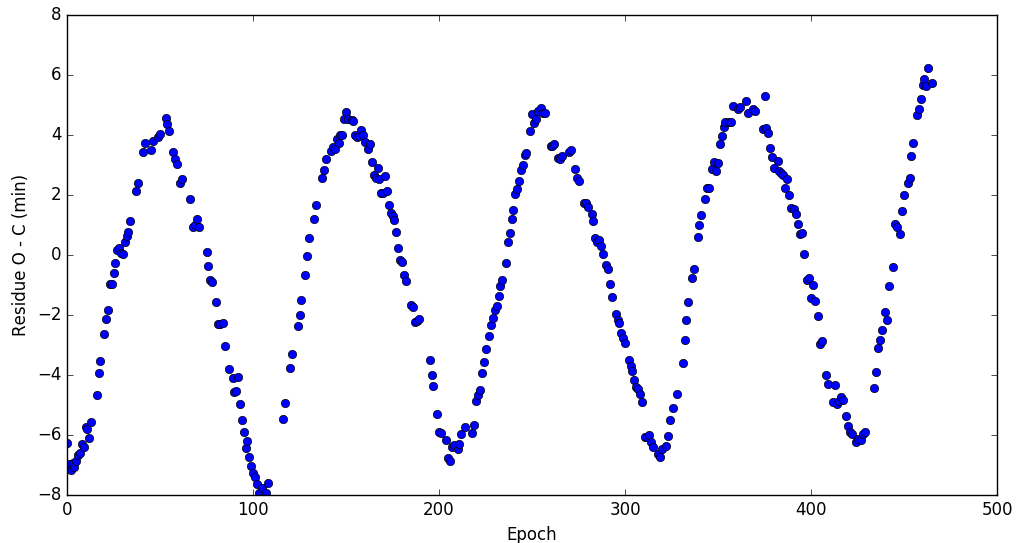
\includegraphics[width=0.95\linewidth]{oc/oc_8719897.png} 
    \caption{O-C diagram of KIC 8719897.} 
    \label{fig:oc:a} 
    \vspace{4ex}
  \end{subfigure}%% 
  \begin{subfigure}[b]{0.5\linewidth}
    \centering
    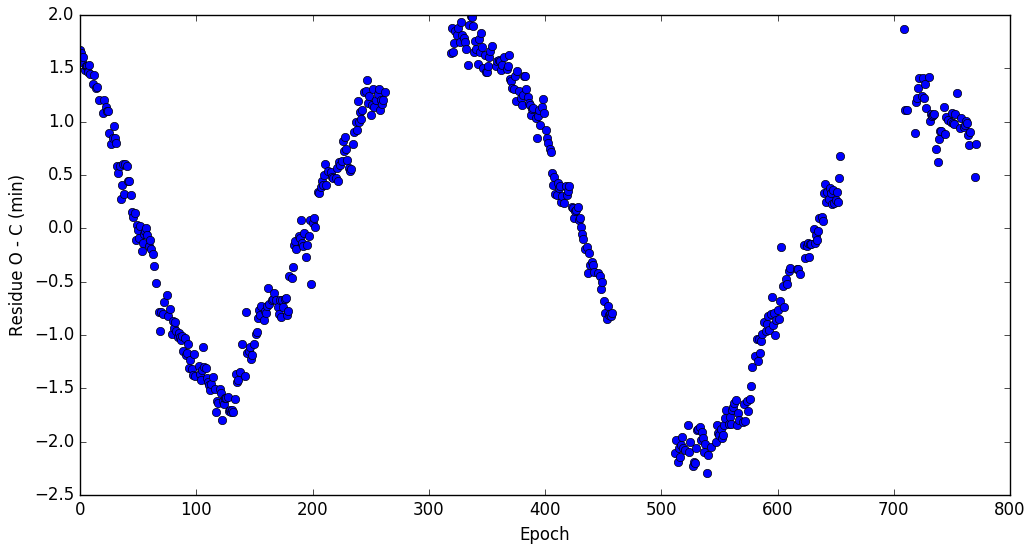
\includegraphics[width=0.95\linewidth]{oc/oc_9912977.png} 
    \caption{O-C diagram of KIC 9912977.} 
    \label{fig:oc:b} 
    \vspace{4ex}
  \end{subfigure} 
  \begin{subfigure}[b]{0.5\linewidth}
    \centering
    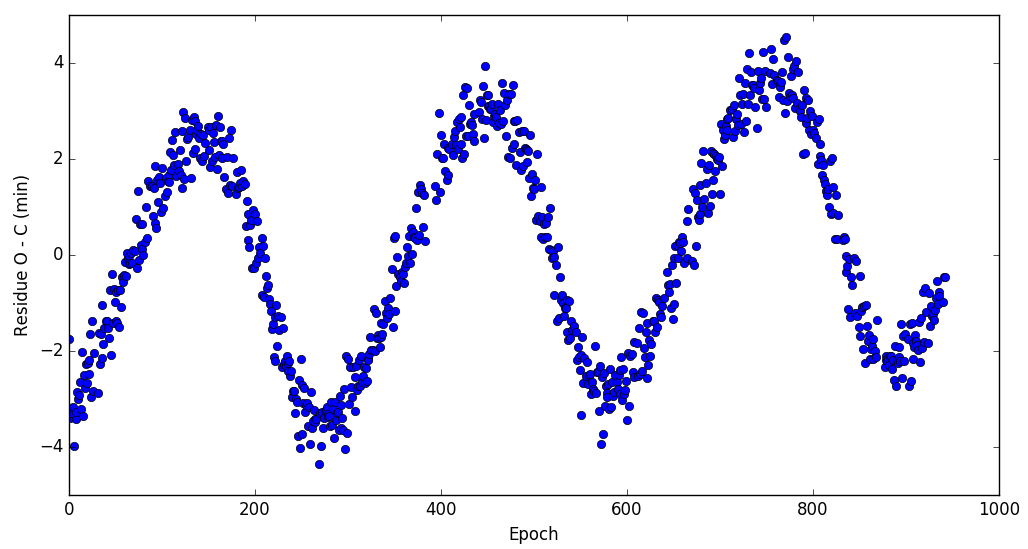
\includegraphics[width=0.95\linewidth]{oc/oc_8043961.png} 
    \caption{O-C diagram of KIC 8043961.} 
    \label{fig:oc:c} 
  \end{subfigure}%%
  \begin{subfigure}[b]{0.5\linewidth}
    \centering
    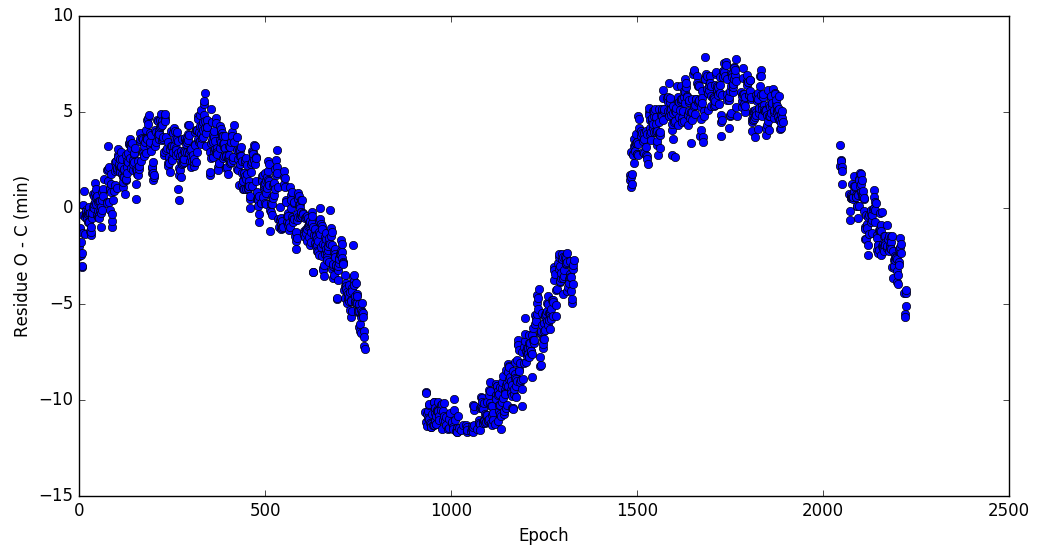
\includegraphics[width=0.95\linewidth]{oc/oc_10226388.png} 
    \caption{O-C diagram of KIC 10226388.} 
    \label{fig:oc:d} 
  \end{subfigure} 
  \caption{Illustration of few obtained O-C diagram with possible presence of 3rd body}
  \label{fig:oc} 
\end{figure}